% NOTES:
%   - Each usage pattern from the literature maps to one step of the generator
%   - Figures are illustrative, similarity/probability values are made up (softmax is computed correctly for T = 0.1)

\begin{frame}{Simulation Methodology: Extending SolidBench}
    \centering
    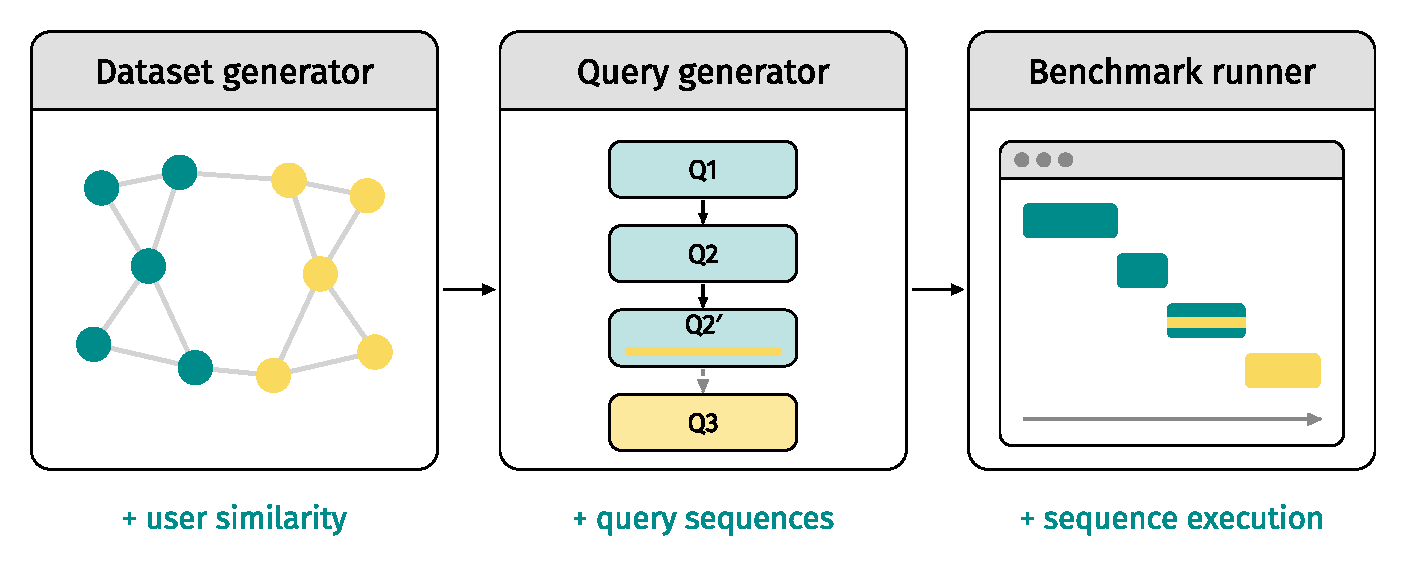
\includegraphics[width=\linewidth]{images/solidbench-extensions.pdf}
\end{frame}

\begin{frame}{Simulation Methodology: Generating a Query Sequence}
    \centering
    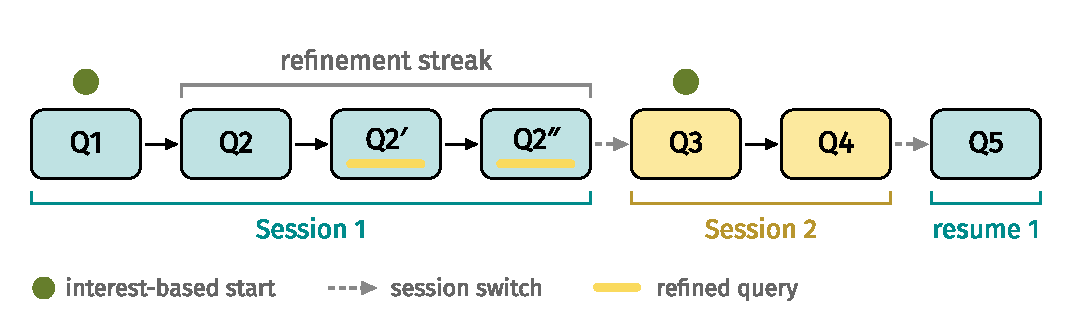
\includegraphics[width=.85\linewidth]{images/sequence-overview.pdf}

    \vspace{0.5em}
    \raggedright
    \begin{itemize}
        \item Each sequence starts from a randomly selected base user
        \item Sessions chain dependent queries, refinement streaks modify them step-by-step
        \item A single seeded random generator keeps sequences reproducible
    \end{itemize}
\end{frame}


\begin{frame}{Usage Pattern: Logical Sessions}
    \begin{columns}[c]
        \begin{column}{0.5\textwidth}
            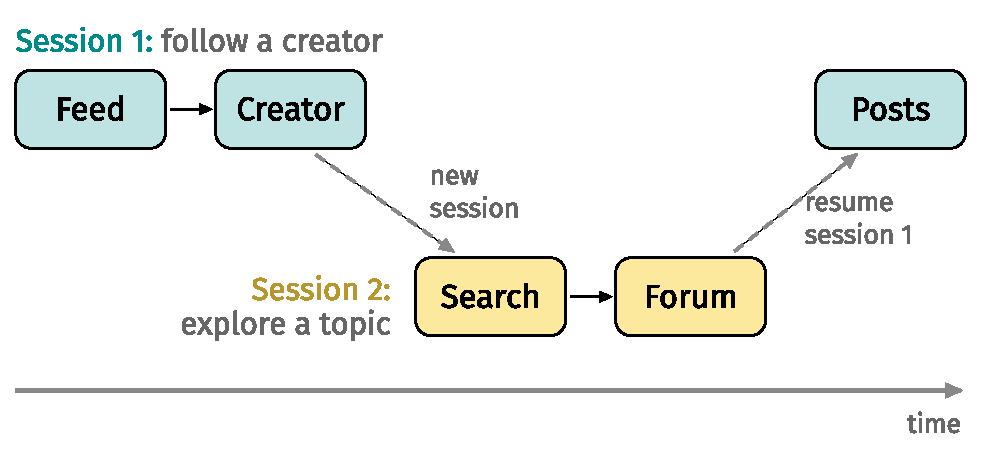
\includegraphics[width=\linewidth]{images/logical-sessions.pdf}
        \end{column}

        \begin{column}{0.5\textwidth}
            \small
            \begin{block}{Observed \parencite{meiss_whats_2009}}
                \begin{itemize}
                    \item Browsing groups into goal-oriented sessions
                    \item New sessions in $\sim$15\% of clicks
                \end{itemize}
            \end{block}
            \begin{block}{Simulated}
                \begin{itemize}
                    \item Next query instantiated from previous results
                    \item Switch to a new session or resume an old one
                \end{itemize}
            \end{block}
        \end{column}
    \end{columns}
\end{frame} 

\begin{frame}{Usage Pattern: User Interests}
    \begin{columns}[T]
        \begin{column}{0.5\textwidth}
            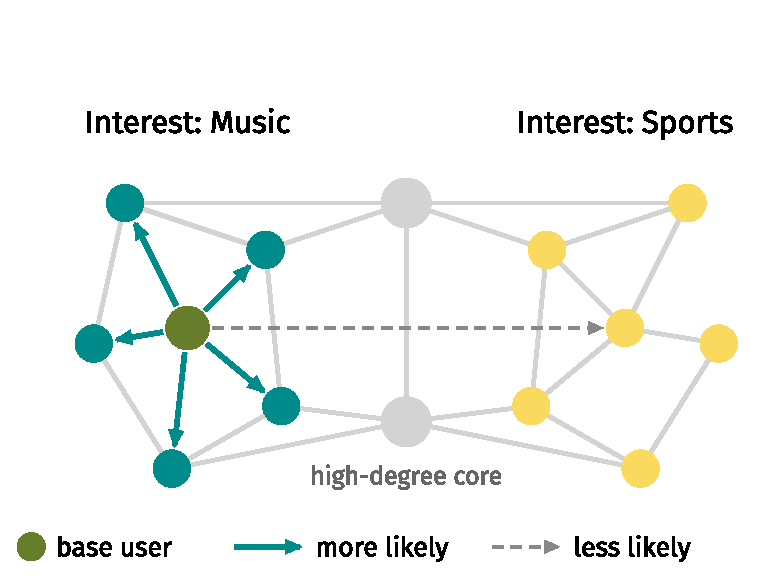
\includegraphics[width=\linewidth]{images/user-interests.pdf}
        \end{column}

        \begin{column}{0.5\textwidth}
            \small
            \begin{block}{Observed \parencite{mislove2007measurement,mitzlaff2013user}}
                \begin{itemize}
                    \item Users form communities around shared interests
                    \item Shared interests drive more interactions
                \end{itemize}
            \end{block}
            \begin{block}{Simulated}
                \begin{itemize}
                    \item User similarity on interests and studies
                    \item Similar users are more likely to start a session
                \end{itemize}
            \end{block}
        \end{column}
    \end{columns}
\end{frame}


\begin{frame}{Usage Pattern: Query Refinement}
    \centering
    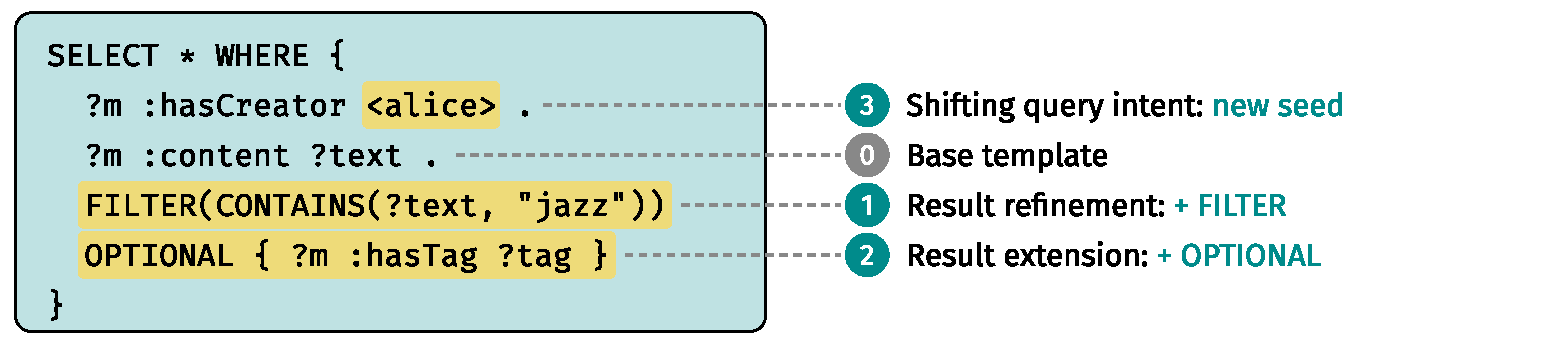
\includegraphics[width=\linewidth]{images/query-refinement-wide.pdf}

    \begin{columns}[T]
        \begin{column}{0.48\textwidth}
            \small
            \begin{block}{Observed \parencite{bonifati2020analytical,arenas2025exploring}}
                \begin{itemize}
                    \item Queries refined step-by-step
                    \item Mostly \texttt{FILTER}, \texttt{UNION}, \texttt{OPTIONAL}
                \end{itemize}
            \end{block}
        \end{column}
        \begin{column}{0.48\textwidth}
            \small
            \begin{block}{Simulated}
                \begin{itemize}
                    \item Composable transformations on queries
                    \item Randomly select sequence of transformations to add to query sequence
                \end{itemize}
            \end{block}
        \end{column}
    \end{columns}
\end{frame}
